\documentclass[a4paper,10pt,twocolumn]{article}
\usepackage{amsmath}
\usepackage{amssymb}
\usepackage{graphicx}
\usepackage{epstopdf}
\usepackage{inputenc}
\usepackage{fullpage}
\usepackage[colorlinks=true,linkcolor=cyan,urlcolor=cyan,citecolor=black]{hyperref}
\usepackage{cleveref}
\usepackage{multirow}

\usepackage{balance}


\renewcommand*\rmdefault{ppl}
\setcounter{secnumdepth}{2} 

\newcommand{\SRL}{\textbf{SRL}}
\newcommand{\Semcor}{\emph{SemCor 3.0}}
\newcommand{\LSTM}{\emph{LSTM}}
\newcommand{\BiLSTM}{\emph{BiLSTM}}
\newcommand{\CELLSIZE}{150}
\newcommand{\GCN}{\emph{GCN}}

%leave more space between rows in table
 \renewcommand{\arraystretch}{1.2}

\begin{document}
\begin{titlepage}
\newcommand{\HRule}{\rule{\linewidth}{0.5mm}}
\center 
\textsc{\LARGE Sapienza University of Rome }\\[2cm] 

\HRule \\[0.4cm]
{ \Huge \textbf {Natural Language Processing}}\\[0.5cm]
{\huge {Third Homework Assignment}}\\[0.4cm]
\HRule \\[1.5cm]

\author{Giorgio Mariani}

\begin{centering}
 \LARGE
\emph{Author:} \\[0.25cm]
Giorgio Mariani
\end{centering} \\[3cm]

\includegraphics[width=7.4cm]{logo.png}
\vfill 
\end{titlepage}
\newpage{}


\section{Problem Description}
The \emph{Semantic Role Labeling} (\SRL) problem \cite{srl} consists in the identification, given a predicate in a sentence, of its semantic arguments (i.e. the words in the sentence which play an important \emph{semantic role} for the predicate, like the \emph{subject} of a certain predicate). More precisely, the \SRL{} problem consists in the identification and subsequent role annotation of  predicate arguments, having a sentence and a semantically disambiguated predicate contained in it. Obviously achieving a good solution for such a problem can open new possibilities for more semantically capable softwares.  It can be expecially useful for tasks like \emph{Question-Answering} and \emph{Information Extraction}.
The goal of this assignment is the implementation of three deep neural network architecture for \SRL{}, heavily inspired by the work of \emph{D. Marcheggiani} and \emph{I. Titov} \cite{simple} \cite{gcn}.
\begin{table}[h!]

\centering
\textbf{Example of \emph{semantic role labeling} of a predicate:}\\~\\
\begin{tabular}{|c|c|c|c|c|c|}\hline
The &cat &is &on &the &table.\\\hline\hline
&\textbf{A0}& \textbf{be.01}&&&\textbf{A1}\\\hline
\end{tabular}

\end{table}

\subsection{State of the Art for \SRL}
At first, when this problem was first proposed, a great deal of importance was given to the syntactic features of words and sentences, labeling syntactic chunks of sentences with the respective semantic role. However, lately the state of the art solutions for this problem  have been progressively moving towards more deep neural network oriented approaches, giving less focus to syntactic information and parsing (leaving responsibility for pattern recognition in the sentence to the network). Specifically, in this assignment two of such models were taken into account: A simple syntactic-agnostic neural model and a more complex one built on top of the first which takes advantage of the sentence's \emph{dependency tree}.


\section{Training and Evaluation Data}
\label{sec:training_data}
The data used for training the neural networks is the \textbf{CoNLL 2009} English \emph{training} dataset.\\
This dataset contains 39,279 sentences, and for each word its \emph{Part-of-Speech}, \emph{lemmatization} and dependency info (\emph{dependency head} word and \emph{dependency type}) are  shown, together with eventual predicate-argument information. 


In order to measure the performance of each neural model the \textbf{CoNLL 2009} English \emph{development} data-set is used. Such data-set contains 1,334 sentences and is structured in the same fashion as the \emph{training} one.


\section{Used Approach}
During the execution of this assignment mainly three neural network models were  considered and  implemented:
\begin{itemize}
\item A relatively simple neural network, mostly composed by a \BiLSTM{} (see \cref{sec:lstm}). It is used as a baseline. This model is a scaled down version of the model presented in \cite{simple}.
\item A deep neural network (built on top of the first one) which exploits dependency information through a \GCN{} (see \cref{sec:gcn}). This model, like the previous one, is a simplified and scaled implementation of an already existing model \cite{gcn}.
\item An alternative neural network architecture exploiting dependency information through a \GCN{}.
\end{itemize}

\subsection{Long Short-Term Memory Neural Networks}
\label{sec:lstm}
\emph{Long Short-Term Memory}\footnote{For a brief explanation follow this \href{http://colah.github.io/posts/2015-08-Understanding-LSTMs/}{link}.} (\LSTM) neural networks are  a useful type of neural networks which is able to work relatively well (compared to simple \emph{RNNs}) over sequences of input data. They are able to do so by utilizing a memory, which is able to propagate information along the sequence (that is the reason of the "Long" part of the name, since information in the first sequence element can effect even the last one).

It is common to stack up different \LSTM{} layers, in order to obtain a more expressive network, and it is especially useful to stack two \LSTM{} and organize them in such a way that the top one receive the reversed output of the bottom one (this type of architecture is called \emph{Binary} \LSTM{} (\BiLSTM)): the main advantage of \BiLSTM{}s is that when computing a word's output  both its left and right context (previous and future words) are considered during the processing, while with standard \LSTM{}s only information coming from the left context can effect the output.


\subsection{Graph Convolutional Neural Networks}
\label{sec:gcn}
\emph{Graph Convolutional Networks}\footnote{More info about \GCN{} \href{https://tkipf.github.io/graph-convolutional-networks/}{here}.} (\GCN)  are a class of neural networks designed for a specific goal:  the elaboration of graph data through a neural network. 
\begin{figure}[h!]
\caption{\GCN{} Example.}
\label{fig:gcn}
\centering
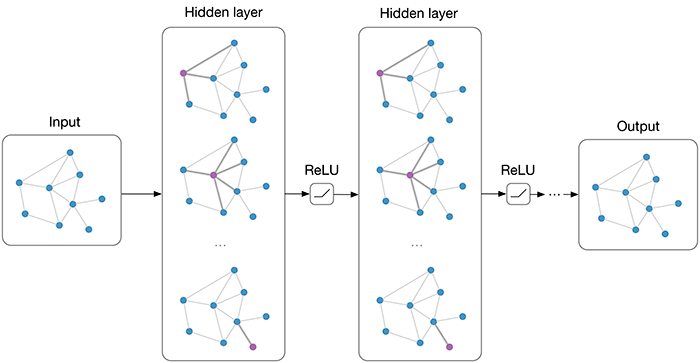
\includegraphics[width=.4\textwidth]{gcn.png}
\end{figure}

\GCN{}s work in the following manner: consider the graph $G = (V,E)$, with $n = |V|$, and with each vertex in the graph having an associated feature vector $x_i$ (with $d$ dimensions), then for all $x_i$ a corresponding output feature vector $z_i$ (with $d'$ dimensions) exists and it is expressed as function of $i$'s neighborhood ($N_i$)  and the vector $x_i$ itself.


There is no golden rule about the shape of such function, however a simple yet effective one could be something similar to
$$
z_i = \mathop{\mathrm{ReLU}}\left(\sum_{j \in N_i	\cup \{i\}} Wx_j + b\right)
$$
\begin{center}
\footnotesize
with $W$ an $n\times d'$  weight matrix and $b$ a bias with  $d'$ dimensions.
\end{center}
Since it uses data from all the node's neighbors and is a non-linear function.

Usually however, more complex operations are also involved in the computation, operators like \emph{gates} and \emph{normalization factors}.

\paragraph{}
Obviously, if only one \GCN{} layer is used then it is not possible, when computing a node's output value, to use information from non-adjacent nodes.
However, by stacking more layers it is possible to reach more and more nodes: with two layers, information between nodes that have distance  two or less can be used, with three, nodes at distance three or less can be used and so on. s

\section{Simple Architecture}
\label{sec:simple_arch}
This model is a simplified and smaller implementation of the neural network described in \cite{simple}. It is composed by mainly three components: a \BiLSTM{} layer, a predicate encoding component and finally a simple \emph{Softmax} classifier layer. The network takes as input a  word sequence\footnote{For sake of simplicity we consider the input to be a single sequence: in truth the network works over batches of such sequences (padded w.r.t. the longest in the batch).} (representing a  sentence), each input word is expressed in the network through the concatenation of the following word-specific data:
\begin{itemize}
\item A pre-trained, non-trainable word embedding of the \emph{lemma} associated to the word (\textbf{GloVe} embeddings with 100 features).
\item A trainable randomly initialized word embedding of the same \emph{lemma} (with 100 dimensions).
\item A trainable randomly initialized embedding of the word's \emph{Part-of-Speech} using 16 features.
\item A trainable randomly initialized embedding of the word's \emph{dependency-type} using 32 dimensions.
\item If the word is a predicate in the sentence (not necessarily the one whose arguments we are predicting) then a trainable randomly initialized embedding of the predicate (64 dimensions). If the word is not a predicate then a default,  neutral embedding is used.
\item A single boolean field with value equals to 1 if the word is the predicate whose semantic roles are being predicted, else equals to 0.
\end{itemize}
The sentence is then given in input to a single \BiLSTM{} layer with two memory cells (one for the forward pass and one for the backward pass) of $\CELLSIZE{}$ elements each. After, the resulting output is "enhanced" with predicate information  and used by a classification layer.\\This  predicate "enhancing"  works as follows: the \BiLSTM{} predicate word representation is simply concatenated to the each word in the \BiLSTM{} output sequence, so to encode the predicate information with the hidden sentence representation. Finally, this encoded sequence is feed to a standard \emph{softmax} classifier in order to predict (for each word) it's role. 


\subsection{Results}
Despite its  simplicity,  this approach is still able to achieve a relatively adeguate performance (\cref{tab:simple_perf}), and the original  implementation \cite{simple}  (which is slightly more complex and with a lot more parameters) is essentially on-par with the current state of the art. 

\begin{table}[h!]
\centering
\begin{tabular}{|c|c|c|}
\hline\hline
 \textbf{Precision} & \textbf{Recall}&\textbf{F1-measure}\\
 0.8411 & 0.7576&0.7972\\
\hline\hline
\end{tabular}
\caption{Performance of the simple model over the \textbf{CoNLL 2009} \emph{development} data.}
\label{tab:simple_perf}
\end{table}
\begin{table}[h!]
	\centering
	\begin{tabular}{cccc}
	&&\multicolumn{2}{c}{\textbf{Predicted Values}}\\
	& &\textit{Positive}&\textit{Negative}\\\cline{3-4}	
	\multirow{2}{1.1cm}{\textbf{Actual Values}} 
	& \textit{Positive}  &\multicolumn{1}{|c|}{10504} & \multicolumn{1}{|c|}{1259}\\\cline{3-4}
	& \textit{Negative} & \multicolumn{1}{|c|}{1983} & \multicolumn{1}{|c|}{180314}\\\cline{3-4}
	\end{tabular}
	\caption{Confusion Matrix}
\end{table}


\section{Dependency GCN Architecture}
\label{sec:gcn_arch}
Despite the relatively good results achieved by the model described in \cref{sec:simple_arch}, an improvement to the network can still be made by exploiting information about the sentences' \emph{dependency  trees} (\cref{fig:dep_tree}): these are structures that implicitly incorporate a important syntactic and (consequently) semantic information.
\begin{figure}[h]
\caption{Dependency Tree Example.}
\label{fig:dep_tree}
\centering
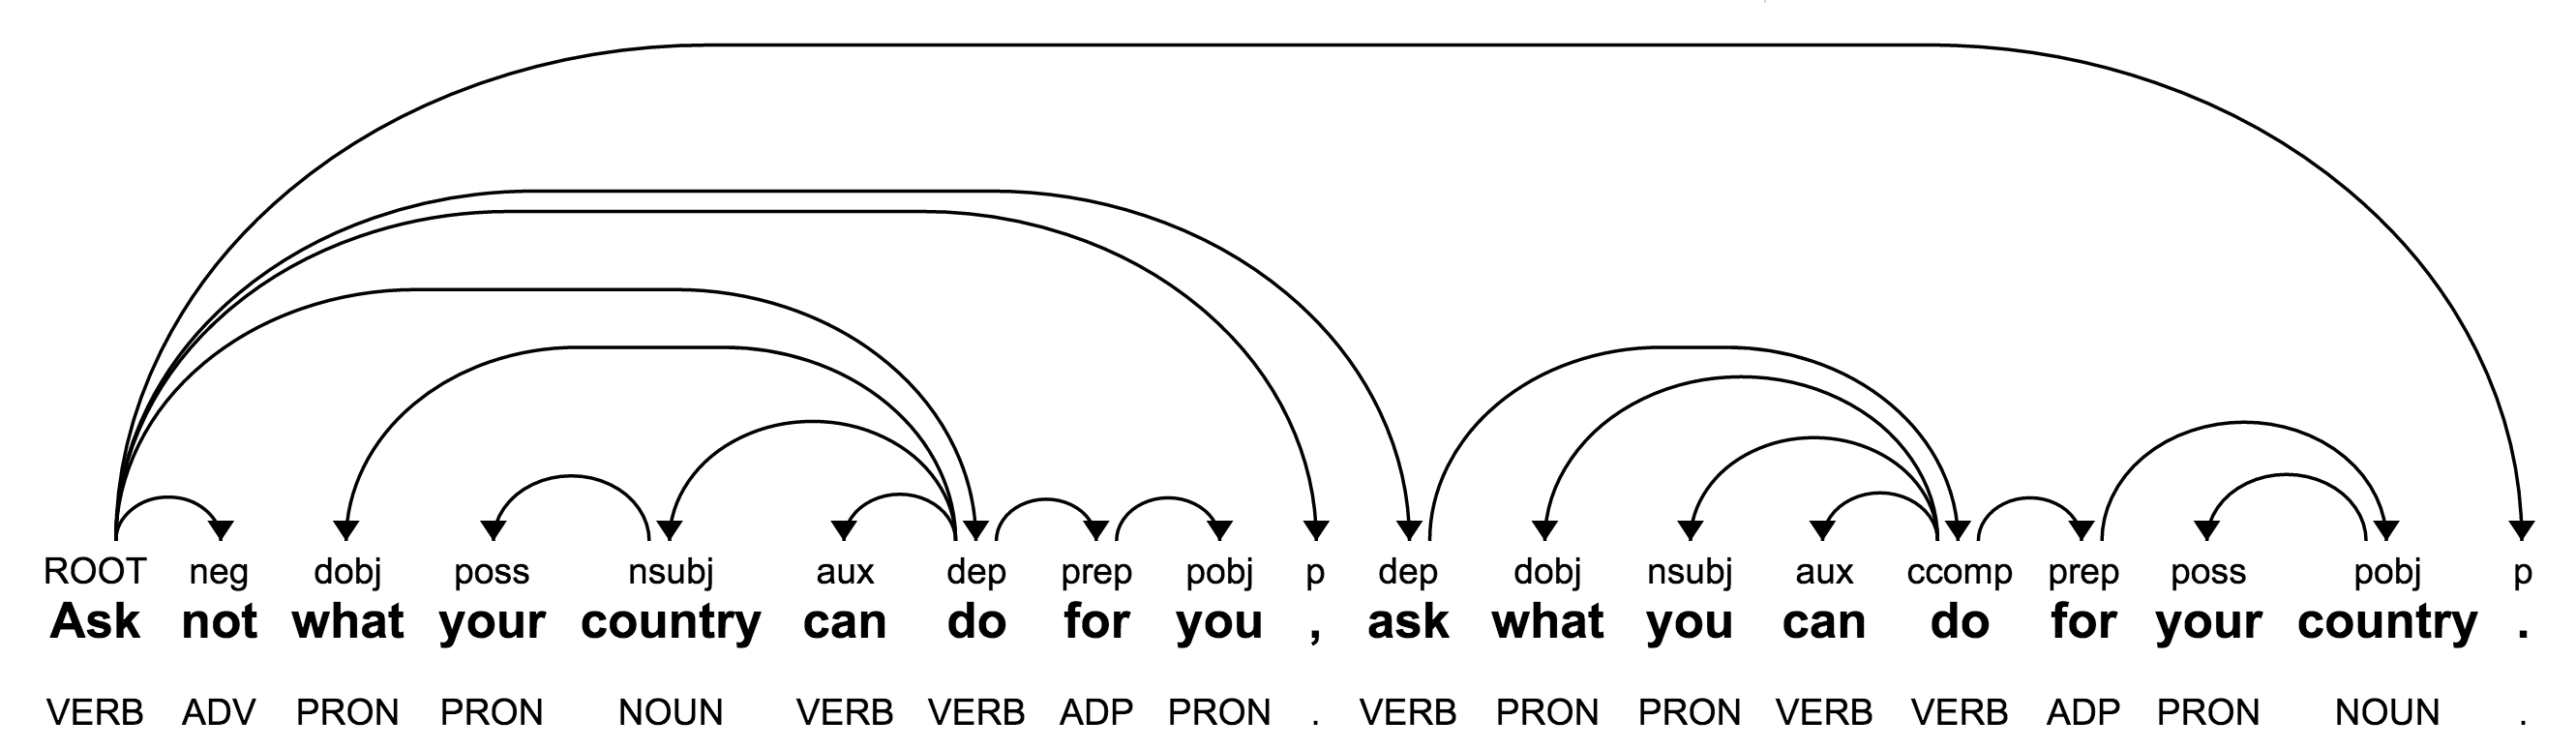
\includegraphics[width=.48\textwidth]{dep_tree.png}
\end{figure}

\paragraph{}
For this reason a model using a specially designed \GCN{}\footnote{Since \emph{dependency trees} are essentially labeled trees, they can be represented through  a \GCN{} architecture. } was developed by \textbf{Marcheggiani} and \textbf{Titov}, built on top of the model presented in \cref{sec:simple_arch}: 

This \GCN{} layer is inserted between the output of the \BiLSTM{} (which is now the \GCN{}'s input) and the predicate extraction/concatenation phase previously described, now working on the \GCN{}'s output.


However, there are some minor problems, namely: how can  dependency info be embedded into the network? And what can be made in order to better control the flow of information between edges? 
\begin{itemize}
\item The solution to the first question consists in the use of \emph{dependency type} specific biases when computing the output of a \GCN{} layer.
\item The addition of edge-specific gates to the \GCN{} answer the second need.
\end{itemize}

We indicate the \emph{dependency type} associated with an edge $(i,j)$ using the notation $L(i,j)$.  It is also useful to differentiate w.r.t.\ the direction of an edge, due to information flowing in the opposite direction  of a syntactic dependency  carrying different information than information going in the same direction, so the edge label is direction-dependant.
For example, consider the arc between \textbf{Ask} and \textbf{not} seen in \cref{fig:dep_tree}:
\begin{align*}
L(\mathrm{Ask},\mathrm{not}) &= \mathrm{neg}_\rightarrow\\
L(\mathrm{not},\mathrm{Ask}) &= \mathrm{neg}_\leftarrow
\end{align*}
Generally speaking, $L(i,j) = \text{dep-type}_{dir(i,j)}$ with
$$
dir(i,j) = 	\begin{cases}
				\rightarrow & \text{if $i$ is the dep. head}\\
				\leftarrow & \text{if $i$ is the dependant}\\
				\end{cases}
$$

The final formulation for the \GCN{} layer function used by is then the following:
$$
z_i = \mathop{\mathrm{ReLU}}\left(\sum_{j \in N_i\cup\{i\}}g_{j,i}\left(W_{dir(i,j)} x_j + b_{L(j,i)}\right)\right)
$$
Where $g_{j,i}$ is a gate that uses edge and vertex information, in order to decide whether to block or allow a certain node.
The precise gate math formulation is: 
$$
g_{j,i} =\sigma \left( \hat{w}_{dir(j,i)}\cdot x_j + \hat b_{L(j,i)} \right)\\ 
$$

\subsection{Results} The addition of this supplementary layer allows for better role predictions when using the network, with a drastic increment of the network's \emph{Recall}.

\begin{table}[h!]
	\centering
	\begin{tabular}{|c|c|c|}
		\hline\hline
		\textbf{Precision} & \textbf{Recall}&\textbf{F1-measure}\\
		0.8524 & 0.82 &0.8359\\
		\hline\hline
	\end{tabular}
	\caption{Performance of the \GCN{} extended architecture over the \textbf{CoNLL 2009} \emph{development} data.}
	\label{tab:gcn_perf}
\end{table}

\begin{table}[h!]
	\centering
	\begin{tabular}{cccc}
		&&\multicolumn{2}{c}{\textbf{Predicted Values}}\\
		& &\textit{Positive}&\textit{Negative}\\\cline{3-4}	
		\multirow{2}{1.1cm}{\textbf{Actual Values}} 
		& \textit{Positive}  &\multicolumn{1}{|c|}{11370} & \multicolumn{1}{|c|}{1474}\\\cline{3-4}
		& \textit{Negative} & \multicolumn{1}{|c|}{1968} & \multicolumn{1}{|c|}{180217}\\\cline{3-4}
	\end{tabular}
	\caption{Confusion Matrix}
\end{table}

\section{Alternative Dependency GCN Architecture}
The model described in \cite{gcn} (\cref{sec:gcn_arch}) works by creating a deep network composed firstly by a \BiLSTM{} layer, then a \GCN{} layer and finally a classifier one. Such network exploits the different nature of \BiLSTM{} and \GCN{} in order to achieve better performance (by complementing layer-specific advantages).

 However, in \cite{gcn} it is never explicitly expressed why the  two layer should be stacked together, for example: why not use these two layers parallelly and then leave to the classifier the decision to whether use the information from the \BiLSTM{} or from the \GCN{}? That is exactly what was experimented during the development of this assignment: an alternative \GCN{}-\BiLSTM{} architecture was created and tested, with relatively good results.

 The input representation is identical to one described in \cref{sec:simple_arch}. However, after the  translation into feature vectors the input sequence is given as input (parallelly) to both a \BiLSTM{} layer (whose output sequence is indicated by $h_{lstm}$) and a \GCN{} layer (having as output the sequence $h_{gcn}$). The same predicate extraction and concatenation shown in \cref{sec:simple_arch} is then applied over both $h^{lstm}$ and $h^{gcn}$.
 
 The major difference of this model is the classifier layer, since it must be able to process the information from both $h^{lstm}$ and $h^{gcn}$.
 Indeed, instead of having a single classification layer, two are used (one for the \BiLSTM{} and one for th \GCN{}) and then a sum (controlled through gates) is applied in order to compute the definite \emph{logits} of the model.
 \begin{align*}
 z^{lstm}_i &= \mathop{h^{lstm}_i} W_{lstm} + b_{lstm}\\
 z^{gcn}_i &= \mathop{h^{gcn}_i} W_{gcn} + b_{gcn}
 \end{align*}
  The actual output of the network (i.e.\ the sequence of \emph{semantic role} probabilities $z$) is then equal to
 $$
 z_i = \mathrm{Softmax}\big(g^{lstm}_{i}\cdot z^{lstm}_i + g^{gcn}_{i}\cdot z^{gcn}_i\big)
 $$
 with  $g^{\alpha}_{i}$ word-specific gates such that 
 $$
 g^{\alpha}_{i} = \sigma ( h^\alpha_i \hat w_\alpha  + \hat b_\alpha)
 $$

\subsection{Results}
This novel architecture achieves even better results than the the previous one (\cref{sec:gcn_arch}), improving both \emph{Precision} and\emph {Recall} of the system. However, is still quite far from achieving \emph{state-of-the-art} performances.
\begin{table}[h!]
	\centering
	\begin{tabular}{|c|c|c|}
		\hline\hline
		\textbf{Precision} & \textbf{Recall}&\textbf{F1-measure}\\
		0.861 & 0.8323 &0.8464\\
		\hline\hline
	\end{tabular}
	\caption{Performance of the alternative dependency \GCN{} model over the \textbf{CoNLL 2009} \emph{development} data.}
	\label{tab:alt_perf}
\end{table}

\begin{table}[h!]
	\centering
	\begin{tabular}{cccc}
		&&\multicolumn{2}{c}{\textbf{Predicted Values}}\\
		& &\textit{Positive}&\textit{Negative}\\\cline{3-4}	
		\multirow{2}{1.1cm}{\textbf{Actual Values}} 
		& \textit{Positive}  &\multicolumn{1}{|c|}{11541} & \multicolumn{1}{|c|}{1334}\\\cline{3-4}
		& \textit{Negative} & \multicolumn{1}{|c|}{1863} & \multicolumn{1}{|c|}{180291}\\\cline{3-4}
	\end{tabular}
	\caption{Confusion Matrix}
\end{table}

\bibliographystyle{unsrt}
\bibliography{mybib}
\end{document}